\documentclass[12pt]{article}

% Language setting
% Replace `english' with e.g. `spanish' to change the document language
\usepackage[english]{babel}

% Set page size and margins
% Replace `letterpaper' with `a4paper' for UK/EU standard size
\usepackage[letterpaper,top=2.5cm,bottom=2.5cm,left=2.5cm,right=2.5cm,marginparwidth=1.75cm]{geometry}

% Useful packages
\usepackage{bm}
\usepackage{multirow} 
\usepackage{afterpage}
\usepackage{amsmath}
\usepackage{booktabs}
\usepackage{graphicx}
\usepackage{indentfirst}
\usepackage{float}
\usepackage{listings}
\usepackage[colorlinks=true, allcolors=blue]{hyperref}
\usepackage{subcaption}
\usepackage{amsfonts}
\captionsetup{compatibility=false}
\title{Scientific Machine Learning for Model Order Reduction of Large Scale Problems \\ \Large Technical Milestone Report}

\author{Honghao Wang \\[0.5cm]{\Small Supervisor: Garth N. Wells, Nirav Vasant Shah}}

\begin{document}
\maketitle

\begin{center}
    \section*{\small Summary}
\end{center}

{\footnotesize This project aims to revolutionise the way in solving partial differential equations (PDEs). Departing from traditional measures reliant on finite element methods, the project proposes a novel approach integrating Model Order Reduction (MOR) with Neural Networks (NN) in building and training a problem-solving model. The project also seeks to develop a simple open-source library for users to achieve such a purpose. }

\section{Introduction}
Solving partial differential equations (PDEs) underpins critical scientific advancements across diverse fields. Nowadays, enhanced computational capabilities combined with improved algorithms allow for high-fidelity numerical solutions to intricate problems using standard discretisation methods. For example, classical methods such as the finite element method (FEM) are used to solve the governing PDE. In this project, we are interested in solving the high-fidelity FEM model repeatedly. However, this could pose very high stress on the limited computational resources because solving high-fidelity models for various parameters usually involves computing a large number of degrees of freedom for the solution. Hence, using the full-order model usually requires access to high-performance computing systems, and the process can be expensive. 

To address the issue, model order reduction (MOR) helps to alleviate the computational burden by identifying a lower dimensional representation of the parametric dependence of the high-fidelity model. The basic idea on which MOR is based is related to the fact that often the parametric dependence of the problem at hand has an intrinsic dimension much lower than the number of degrees of freedom associated to the governing high-fidelity solution \cite{shah2022finite}. There are two stages in an MOR procedure. The first one is an offline stage. During this stage, a large number of solution manifolds (solved under different initialisations of parameters) are collected together to form a solution snapshot matrix. The MOR algorithm can then be run on the snapshot matrix, which identifies the most significant modes that form the reduced basis space. Stage two is an online stage where information regarding the reduced basis space is fully utilised, which allows for the computing of the projections of new high-fidelity solutions onto the lower intrinsic dimensions. 

This project focused on the mixed formulation for the Poisson equation, which included an extra vector term $\sigma$ that represented the flux of the scalar field in the Poisson equation. The parametrisation of PDEs incorporated changing variables in the governing equations that allowed for more flexibility in the system. In this report, we explain the choices of the parameters through the MOR results. 

We aim to develop a framework for data-driven MOR by combining Proper Orthogonal Decomposition (POD) with Artificial Neural Networks (ANN). The method involves identifying reduced basis space by performing POD (with the RBniCSx package), training the ANN with snapshots of PDE solutions as inputs, and using the trained ANN for a quick approximation of the solution field of a PDE. While offering data-driven efficiency and reducing reliance on high-fidelity FEM models, the trade-offs include a sacrifice in accuracy and extended training times for the ANN. The loss in accuracy was particularly evident in the vector field. Achieving a balance between accuracy and efficiency is crucial for the successful implementation of this approach.

To accelerate the runtime of the programme, this project leverages supercomputers through data-parallel computing, which divides tasks into smaller sub-tasks, allowing multiple processors to simultaneously execute computations. Both CPU and GPU-based parallelisation were utilised in the project. The CPU-based parallelisation involves distributing the computational workload across multiple CPU cores to accelerate the generation of data. This involves solving large-scale PDEs with the FEM library FEniCSx, specifically for computing the reduced basis functions in POD and for obtaining the ANN training data; In the context of ANN training, the GPU-based parallelisation was utilised with the help of TensorFlow. Partitions of the dataset are distributed to individual processors, each handling its subset of the dataset. Through distributed ANN training, parallel processing accelerates the learning process. The outputs during each training epoch (e.g. losses and gradients) are synchronised among processors. 

\textcolor{red}{Add the figure \ref{fig:project_explain} with explanation?}

\begin{figure}[!h]
    \centering
    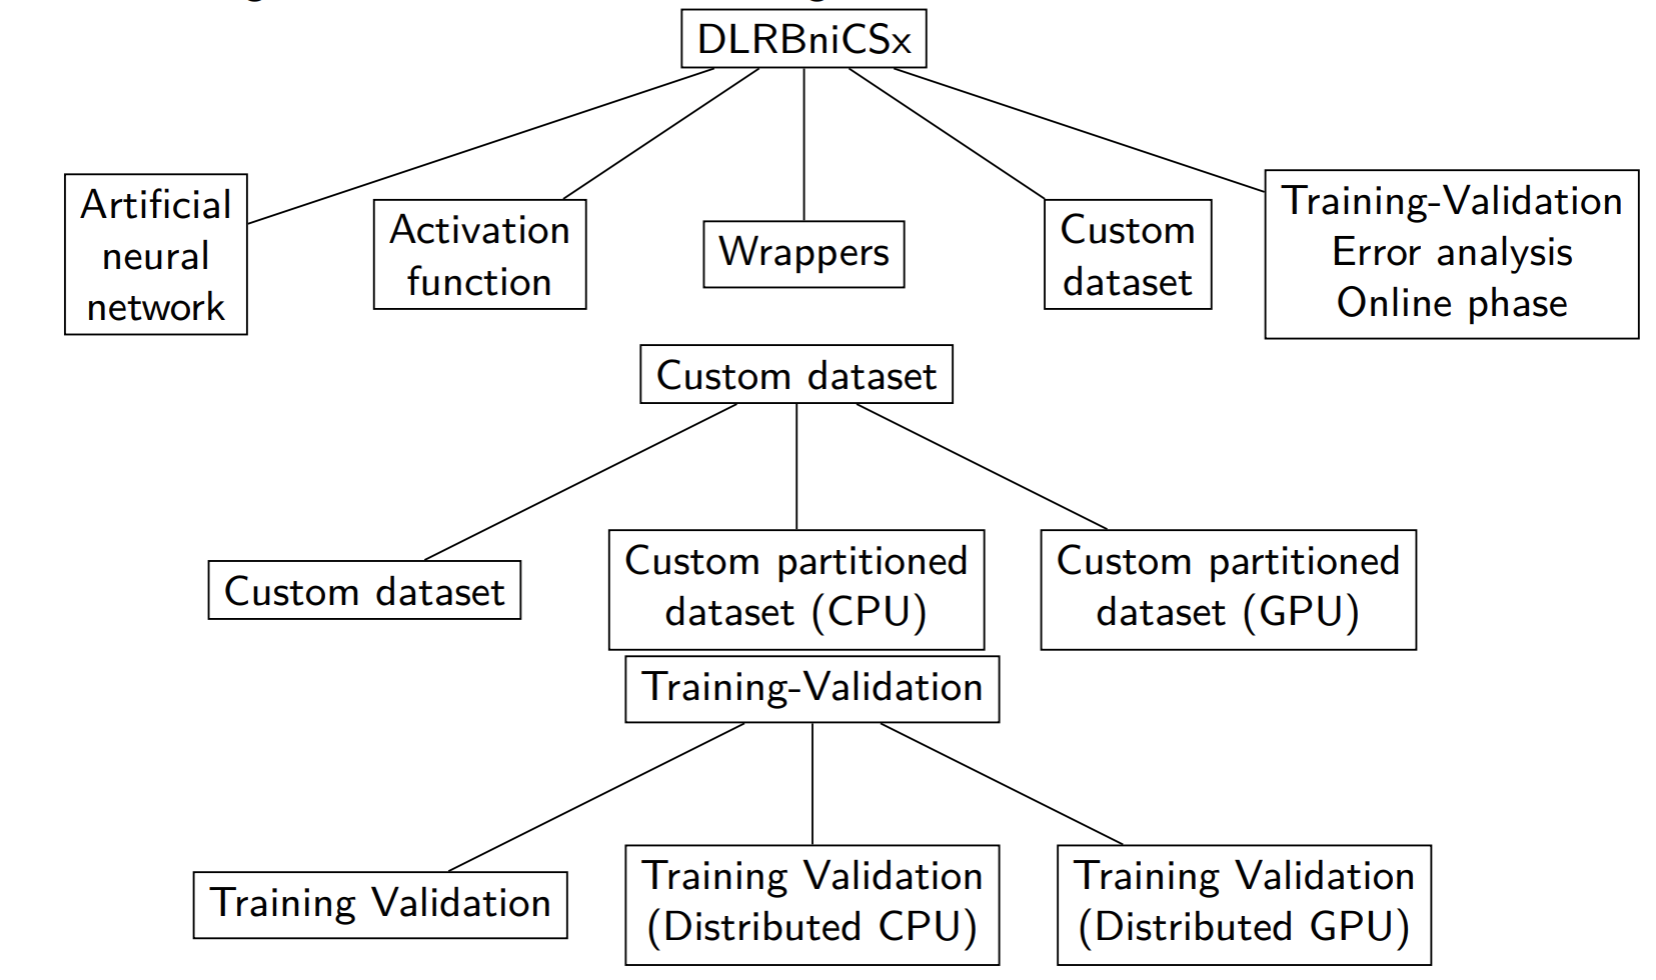
\includegraphics[width=0.7\linewidth]{parallel_fig/project_explain.png}
    \caption{Project outline}
    \label{fig:project_explain}
\end{figure}

Below is a summary of the workflow of this project, which will be discussed in greater depth in this report. In Section 2, we will introduce the governing equation of the mixed formulation for the Poisson equation and how the traditional finite element method is used to solve for the full-order solution. Section 3 focuses on the concept of parametrised 
PDEs and explain our choices of parameters focused on the project. In Section 4, the idea of MOR is explained in detail, and we will discuss the result and the effectiveness of MOR in reducing dimensionality, along with a detailed explanation of the choice for parameterisation. The use of ANN will then be covered in Section 5, followed by a presentation of the numerical results in Section 6. Lastly, the concept of both GPU and CPU parallelization is covered in Section 7.  

\begin{comment}
\begin{enumerate}
    \item \textbf{POD-ANN training phase:}
        \begin{enumerate}
            \item Use FEM to compute the sample solutions with different input parameters and obtain the snapshot matrix (incorporating parallelisation);
            \item Perform POD on the snapshot matrix to obtain the reduced basis space;
            \item Project the sample solutions on a reduced basis to obtain the training data;
            \item Train the ANN with the training dataset (incorporating parallelisation).
        \end{enumerate}

    \item \textbf{Prediction phase:}
        \begin{enumerate}
            \item Insert the input parameters to the trained ANN and obtain the predicted output on the reduced basis function space;
            \item Reconstruct the high-fidelity solution from the reduced basis output and the reduced basis functions.
        \end{enumerate} 
\end{enumerate}
%%%
\end{comment}

\newpage
\section{Governing Equation and Finite Element Methods}
The Finite Element Method(FEM) is a numerical method for approximating the solution of the governing PDE by discretising the problem domain into smaller elements. Over the discredited domain, the solution is approximated using piecewise polynomial functions. The weak formulation converts the PDE into an equivalent variational form. The general method of weak formulation involves multiplying the PDE by a test function $v$ and integrating it over the domain $\Omega$, which would allow us to perform integration by parts on those terms with second-order derivatives, simplifying the solution process.

Work has been done on some PDEs such as the linear/non-linear Poisson equations, the Navier-Stokes equations etc. In this project, the problem of interest is the mixed formulation for the Poisson equation, which introduces an additional vector variable to represent the gradient of the scalar unknown, namely the (negative) flux, leading to the new PDE:

\begin{align}
    \Vec{\sigma} - \nabla u = 0 \quad \text{, in }\Omega    \label{eqn:PDE1}\\  
    \nabla \cdot \Vec{\sigma} = -f \quad \text{, in }\Omega     \label{eqn:PDE2}
\end{align}

Subject to the Neumann  and Dirichlet boundary conditions:
\begin{align}
     \Vec{\sigma}  \cdot \Vec{n} =  g \quad \text{, on }\Gamma_{N} \label{eqn:boundary1} \\
     u = u_0 \quad \text{, on }\Gamma_{D}   \label{eqn:boundary2}
\end{align}

Here $u$ and $\Vec{\sigma}$ are the scalar and the flux terms, and $\Vec{n}$ is the outward pointing normal vector on the boundary.

Since FEniCSx is implemented based on the FEM, the first step is to convert the PDE into its variational form. Multiplying Equation \ref{eqn:PDE1} and \ref{eqn:PDE2} by test functions $\vec{\tau}$ and $v$, and integrating the gradient term by parts in the first equation, the following variational form is obtained:

\begin{equation}
\int_{\Omega} (\vec{\sigma} \cdot \vec{\tau} + \nabla \cdot \vec{\tau} \, u) \, d\Omega = \int_{\Gamma} \vec{\tau} \cdot \vec{n} \, u \, ds \quad \forall \vec{\tau} \in \Sigma
\end{equation}

\begin{equation}
\int_{\Omega} \nabla \cdot \vec{\sigma} \, v \, d\Omega = - \int_{\Omega} f \, v \, d\Omega \quad \forall v \in V
\end{equation}

Inserting the boundary conditions from equation \ref{eqn:boundary1} and \ref{eqn:boundary2}, we can obtain the following equation to be solved for $(\vec{\sigma}, u) \in \Sigma_g \times V$:

\begin{equation}
    \int_{\Omega} \vec{\sigma} \cdot\vec{\tau} + \nabla \cdot \vec{\tau} \, u + \nabla \cdot \vec{\sigma} \, v  dx = -\int_{\Omega} f v \, dx + \int_{\Gamma_{D}} u_0 \vec{\tau} \cdot \vec{n}  ds
    \label{eqn:variational_form}
\end{equation}

Where $\Sigma_g = \{\vec{\tau} \in H(\text{div}) \text{ such that } \vec{\tau} \cdot \vec{n}|_{\Gamma_N} = g\}$ and $V = L^2(\Omega)$. To discretise the formulation in equation \ref{eqn:variational_form} for FEM to work properly and stably, we used the  Brezzi-Douglas-Fortin-Marini function space with a polynomial degree of $k$ to represent $\Sigma$, and the Discontinuous Galerkin (DG) space with a degree of $k-1$ to represent $V$. The BDMCF space is defined on each mesh element and is designed to provide accurate approximations for vector quantities. The DG space allows discontinuities in the solution between neighbouring elements, making it particularly useful for problems with rapid changes or sharp gradients.  Listing 1 shows the example codes for defining the geometric function space of a mixed-formulation problem. In particular, we have set up a function space \textbf{V}, which is created by mixing the vector and scalar elements. The vector component (flux) \textbf{Q\_el} rests on a BDM element, and the scalar \textbf{P\_el} rests on DG space. 

\begin{lstlisting}[frame=single, caption={Defining geometric parameters / Creating function space }]
Q_el = basix.ufl.element("BDMCF", domain.basix_cell(), k)
P_el = basix.ufl.element("DG", domain.basix_cell(), k - 1)
V_el = basix.ufl.mixed_element([Q_el, P_el])
V = fem.functionspace(domain, V_el)
\end{lstlisting}

The problem is defined and solved with code listing 2, where a LinearProblem object that brings everything together is created. The weak forms \textit{a} and \textit{L} define the PDE, \textit{bcs} includes the functions defining the boundary conditions. Special attention is drawn to the \textit{petsc\_options}, which specifies that the LU decomposition is used as a linear solver. The choice of solvers significantly impacts the efficiency and accuracy of solving linear systems in finite element simulations. Direct solvers like the LU decomposition in this case provide accurate solutions for smaller systems but may become computationally expensive as the problem size increases. Iterative solvers are also commonly found in linear problems, examples include the Conjugate Gradient (CG) or Generalized Minimal Residual (GMRES). They are suitable for large, sparse linear systems, but they are usually more complicated and require pre-conditioning to improve convergence.

\begin{lstlisting}[frame=single, caption={Defining and solving the porblem}, basicstyle=\scriptsize]
problem = fem.petsc.LinearProblem(a, L, bcs=bcs, 
                                  petsc_options={"ksp_type":"preonly","pc_type":"lu"})
w_h = problem.solve()   # solution manifold containing u and sigma
\end{lstlisting}

\vspace{1cm}

\textcolor{red}{Model discussion on mesh choices? size of discretisation? Function spaces}

\newpage
\section{Proper Orthogonal Decomposition for MOR}

To perform MOR before passing the data to training the NN, proper orthogonal decomposition(POD) is used with the facilitation by the RBniCSx package. In particular, upon receiving the PDE data snapshot matrix, singular value decomposition is performed, which allows us to pick the most significant singular values and their related modes. Detailed codes of this part have been compiled before the start date of this project, but they have been thoroughly studied to integrate them with the NN building packages for development purposes. 
\section{Project Plans and Conclusion}

By the end of the day, the goal of the project is to combine lots of aforementioned concepts to create a simple and efficient library for conveniently solving PDEs through the training of an NN. Since many concepts were relatively new, the Michaelmas term was mainly spent on preliminary work. Over the Christmas holiday, rather more investigations were made on the mixed formulation for the Poisson equation and POD for MOR. Lots of works were done but some were too trivial to be discussed as a single section, but will be listed below. By the start of the lent term, the following progress has been made on the project:

\begin{itemize}
    \item Preliminary reading on MOR techniques and code implementation of POD with collected snapshots through RBniCSx
    \item Familiarization with FEniCSx on defining different types of PDEs, different solvers, function spaces, and exploration of the effects of parameters in the mixed formulation.
    \item Parallel data partitioning and scaling functions with MPI used for parallel training. 
    \item Familiarization with distributed training with TensorFlow
    
    % Elaboration can be added here
\end{itemize}

The plan for the next few months is to combine what has been studied and produce a more complete Python library for performing NN training on solving different PDEs, and to evaluate the performance. Details of the work to be done include:

\begin{itemize}
    \item Integrate open-source libraries to provide Tensorflow support in DLRBniCSx
    \item Implement training-validation procedures on the NN
    \item Compile additional functions, including checkpointing and error analysis
\end{itemize}



\bibliographystyle{alpha}
\bibliography{reference}

\end{document}
